\documentclass{article}

\usepackage[utf8]{inputenc}
\usepackage[slovak]{babel}
\usepackage[a4paper, total={15cm, 22cm}]{geometry}
\usepackage{graphicx}

\begin{document}

	%---------------------------------
	% Titulná strana
	%---------------------------------
	\begin{titlepage}
		\centering
		
\includegraphics[scale=0.1]{images/vut-fit-logo.png} \\
		\vspace{5cm}
		\Huge{FITKit 2: Dekodér morzeovej abecedy} \\
		\vspace{1cm}
		\Large{Dokumentácia} \\
		\vspace{4cm}
		\large{Jozef Hruška} \\
		\vspace{0.5cm}
		\normalsize{\today} \\
		\vfill
		Mikroprocesorové a vestavěné systémy
	\end{titlepage}
	
	%---------------------------------
	% Obsah
	%---------------------------------
	\tableofcontents
	\clearpage
	
	%---------------------------------
	% Popis
	%---------------------------------
	\section{Popis}
	Dekodér morseovej abecedy implementovaný na Platforme FITKit 2. Aplikácia podporuje dekódovanie všetkých znakov anglickej abecedy a číslic 0 až 9, ukladanie až 16 dekódovaných znakov, zmazanie posledného dekódovaného znaku, zmazanie všetkých uložených znakov a nastavenie štyroch dĺžiek doby potrebnej pre rozoznanie znaku - (dash). \\\\
	Na prvom riadku displeja platformy FITKit 2 sú zobrazované už preložené znaky a na druhom riadku je zobrazená sekvencia práve zadávaných znakov morseovej abecedy.
	
	\begin{figure}[h]
		\centering
		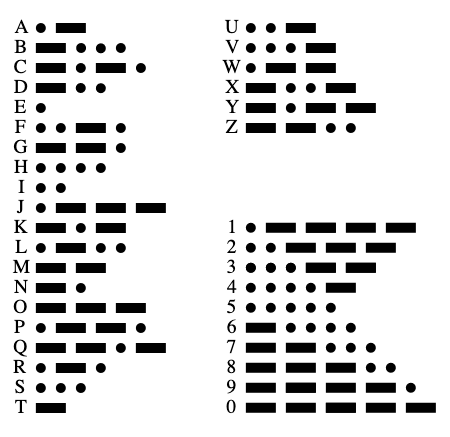
\includegraphics[scale=0.6]{images/supported-signs.png} \\
		\caption{Znaky podporované dekodérom}
	\end{figure}
	
	%---------------------------------
	% Ovládanie
	%---------------------------------
	\section{Ovládanie}
	Ovládanie aplikácie je výhradne pomocou klávesnice na platforme FITKit 2.
	\begin{itemize}
	    \item * - Klávesa pre zadávanie znakov.
	    \item 0 - Klávesa pre zmazanie posledného dekódovaného znaku.
	    \item \# - Klávesa pre zmazanie všetkých uložených znakov.
	    \item A - Rýchlosť 1 (Najrýchlejšia)
	    \item B - Rýchlosť 2
	    \item C - Rýchlosť 3
	    \item D - Rýchlosť 4 (Najpomalšia)
	\end{itemize}
	
	%---------------------------------
	% Implementácia
	%---------------------------------
	\section{Implementácia}
	\subsection{Časovač}
	Pri rozpoznávaní, či užívateľ zadal znak '.' alebo '-' je časovač nastavený na aktuálnu rýchlosť nastavenú klávesami A až D. Pri prvotnej inicializácii aplikácie je prednastavená rýchlosť 2 (klávesa B). V prípade že užívateľ zadá jeden zo znakov '.' alebo '-' je ihneď spustený časovač, ktorý ak nie je prerušený spustí obsluhu dekódovania sekvencie znakov morseovej abecedy.
	
	\subsection{Dekodér}
	Po uplynutí časovača pre dekódovanie znaku obsluhujúca rutina porovná sekvenciu znakov so všetkými definovanými znakmi morseovej abecedy a v prípade, že nájde zhodu pridá znak do reťazca už preložených znakov, a obnoví displej.
	
	%---------------------------------
	% Záver
	%---------------------------------
	\section{Záver}
	Implementácia projektu prebiehala bez problémov. Projekt implementuje všetky body zadania a pridáva funkcionalitu zmazania všetkých znakov. Pre efektívnejšie použitie aplikácie projekt využíva možnosti dvojriadkového displeja a preto zobrazuje naraz zadávané znaky aj už znaky už preložené. Pri implementácií bol kladený dôraz aj na efektívnosť kódu.

\end{document}
